\documentclass{article}

\usepackage{/home/paul/Workspace/build/macros}


\title{Annale 2022: corrigé}
\date{}
\author{Paul Catala}


\begin{document}
\maketitle

\section{Optimisation numérique}

\subsection{Méthode de Newton-Raphson}

\begin{enumerate}
	\item On considère la fonction objectif $J(x,y) = \displaystyle \frac{1}{2}x^2 + \frac{9}{2}y^2 - x - 18y + 20$.
	
	Le gradient $\nabla J$ de $J$ au point $(x,y)$ est défini comme le vecteur
	\eq{
		\nabla J(x,y) = \begin{bmatrix} \partial_1 J(x,y) \\ \partial_2J(x,y) \end{bmatrix}.
	}
	où $\partial_1 J$ et $\partial_2 J$ sont les dérivées partielles de $J$ par rapport à $x$ et $y$ respectivement.
	
	La dérivation par rapport à $x$ donne $\partial_1 J(x,y) = x-1$.
	
	La dérivation par rapport à $y$ donne $\partial_2 J(x,y) = 9y-18$.
	
	Le gradient du critère est  donc finalement
	\eq{
		\nabla J(x,y) = \begin{bmatrix} x-1 \\ 9y-18 \end{bmatrix}.
	}
	
	\item La matrice hessienne $\nabla^2 J$ de $J$ en $(x,y)$ est définie comme
	\eq{
		\nabla^2 J(x,y) = \begin{bmatrix} \partial_{11} J(x,y) & \partial_{12} J(x,y) \\ \partial_{21} J(x,y) & \partial_{22} J(x,y) \end{bmatrix}.
	}
	Les dérivées partielles secondes $\partial_{11} J$ et $\partial_{12} J$ s'obtiennent en dérivant $\partial_{1} J$ par rapport à $x$ et $y$ respectivement; les dérivées partielles secondes $\partial_{21} J$ et $\partial_{22} J$ s'obtiennent de même à partir de $\partial_{2} J$.
	
	La matrice hessienne est donc finalement
	\eq{
		\nabla^2 J(x,y) = \begin{bmatrix} 1 & 0 \\ 0 & 9\end{bmatrix}.
	}
	
	\item Une itération de l'algorithme de Newton à partir d'un point $(x_0,y_0)$ fournit un nouveau point $(x_1,y_1)$ défini par la règle de mise à jour suivante
	\eq{
		\begin{bmatrix} x_1 \\ y_1 \end{bmatrix} = \begin{bmatrix} x_0 \\ y_0 \end{bmatrix} - \alpha \nabla^2 J(x_0,y_0)^{-1} \nabla J(x_0,y_0)
	}
	où $\alpha > 0$ est un pas à choisir. Ici $\nabla^2 J(x_0,y_0)$ est une matrice diagonale avec des entrées strictement positives, elle est donc bien inversible (déterminant non nul), et son inverse est simplement donné par
	\eq{
		\nabla J^2(x_0,y_0)^{-1} = \begin{bmatrix} 1 & 0 \\ 0 & \frac{1}{9} \end{bmatrix}.
	}
	En utilisant les formules trouvées aux question précédentes, on obtient donc
	\eq{
		\begin{bmatrix} x_1 \\ y_1 \end{bmatrix} = \begin{bmatrix} x_0 \\ y_0 \end{bmatrix} - \al \begin{bmatrix}1 & 0 \\ 0 & \frac{1}{9}\end{bmatrix} \begin{bmatrix} x-1 \\ 9y-18 \end{bmatrix} = \begin{bmatrix} x_0 \\ y_0 \end{bmatrix} - \al \begin{bmatrix} x_0-1 \\ y_0-2 \end{bmatrix},
	}
	soit, coordonnée par coordonnée
	\eq{
		\left\{\begin{aligned}
			&x_1 = (1-\al)x_0 + \al\\
			&y_1 = (1-\al)y_0 + 2\al
		\end{aligned}\right.
	}
	
\item La fonction $J$ est (strictement) convexe car sa Hessienne est définie positive (valeurs propres strictement positives). Elle admet donc un unique minimiseur, qui satisfait la condition d'optimalité de premier ordre
\eq{
	\nabla J(x_\star,y_\star) = \begin{bmatrix} 0 \\ 0 \end{bmatrix}.
}
c'est-à-dire
\eq{
	\left\{\begin{aligned}
		&x_\star-1 = 0\\
		&9y_\star-18 = 0\\
	\end{aligned}\right.
	%
	\iff
	%
	\left\{\begin{aligned}
		&x_\star = 1\\
		&y_\star = 2 \\
	\end{aligned}\right..
}

On remarque que ce minimiseur est atteint en une seule itération lorsque le pas $\alpha$ est choisi égal à $1$.

\item La valeur du critère au minimum est 
\eq{
	J(1,2) = \frac{1}{2} + 4\frac{9}{2} - 1 - 36 + 20 = \frac{3}{2}.
}

\end{enumerate}


\subsection{Formulation d'un problème d'optimisation}

\begin{enumerate}
	\item Les variables du problèmes sont les dimension $x,y$ et $z$ du parallélépipède. Le critère à minimiser est la surface $S(x,y,z) = 2(xy+yz+xz)$ du parallélépipède, et les contraintes sont celles du volume fixe $V = xyz = 1$ et de positivité des dimensions. On obtient donc le problème suivant
	\eq{
		\min 2(xy+xz+yz) \qscq \left\{\begin{aligned}
			&x > 0\\
			&y > 0\\
			&z > 0\\
			&xyz = 1
			\end{aligned}\right..
	}
	
	\item La contraite de volume fixe impose $\displaystyle z = \frac{1}{xy}$ (valable car $xy > 0$). En réinjectant, on obtient le problème à deux variables suivant
	\eq{
		\min 2(xy+\frac{1}{y}+\frac{1}{x}) \qscq \left\{\begin{aligned}
			&x > 0\\
			&y > 0\\
			\end{aligned}\right..
	}
\end{enumerate} 

\section{Classification}
\subsection{SVM à noyau}

\begin{enumerate}
	\item Le jeu de données est le suivant:
	\bigbreak
	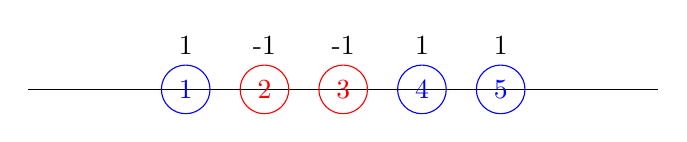
\begin{tikzpicture}
		\draw (-4,0) -- (4,0);
		
		\node[circle,blue,draw,label=1] at (-2,0) {1};
		\node[circle,red,draw,label=-1] at (-1,0) {2};
		\node[circle,red,draw,label=-1] at (0,0) {3};
		\node[circle,blue,draw,label=1] at (1,0) {4};
		\node[circle,blue,draw,label=1] at (2,0) {5};
	\end{tikzpicture}
	
	\item La séparabilité linéaire signifie ici que les deux classes sont de par et d'autre d'un point. Ce n'est pas le cas ici: les deux classes ne sont pas linéairement séparables.
	
	\item L'hyperplan suivant conduit à une erreur de classification, ce qui est bien le nombre minimal d'erreurs:
	\bigbreak
	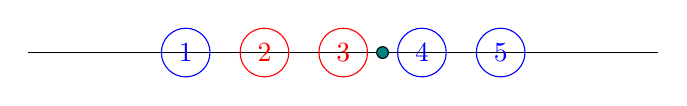
\begin{tikzpicture}
		\draw (-4,0) -- (4,0);
		
		\node[circle,blue,draw] at (-2,0) {1};
		\node[circle,red,draw] at (-1,0) {2};
		\node[circle,red,draw] at (0,0) {3};
		\node[circle,fill=teal,draw,inner sep=1.5pt] at (0.5,0) {};
		\node[circle,blue,draw] at (1,0) {4};
		\node[circle,blue,draw] at (2,0) {5};
	\end{tikzpicture}
	
	\item 
	\begin{enumerate}
		\item On a
		\eq{
			Z = \Phi(X) = \begin{bmatrix} X & X \odot X \end{bmatrix} = \begin{bmatrix} -2 & 4 \\ -1 & 1 \\ 0 & 0 \\ 1 & 1 \\ 2 & 4 \end{bmatrix}.
		}
		
		\item Graphiquement:
		\bigbreak
		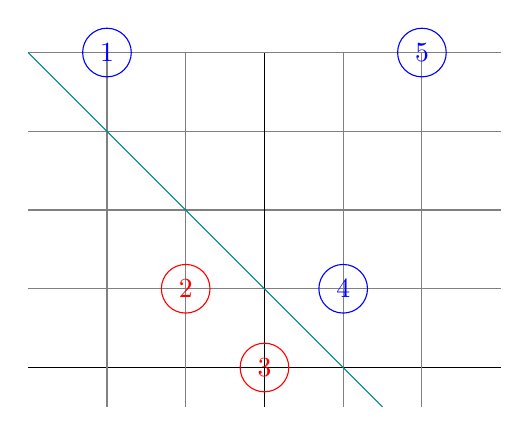
\begin{tikzpicture}
		\draw (-3,0) -- (3,0);
		
		\draw[gray] (-3,1) -- (3,1);
		\draw[gray] (-3,2) -- (3,2);
		\draw[gray] (-3,3) -- (3,3);
		\draw[gray] (-3,4) -- (3,4);
		
		\draw[gray] (-2,-0.5) -- (-2,4);
		\draw[gray] (-1,-0.5) -- (-1,4);
		\draw  (0,-0.5) -- (0,4);
		\draw[gray] (1,-0.5) -- (1,4);
		\draw[gray] (2,-0.5) -- (2,4);
		
		\draw[teal] (-3,4) -- (1.5,-0.5);
		
		\node[circle,blue,draw] at (-2,4) {1};
		\node[circle,red,draw] at (-1,1) {2};
		\node[circle,red,draw] at (0,0) {3};
		\node[circle,blue,draw] at (1,1) {4};
		\node[circle,blue,draw] at (2,4) {5};
	\end{tikzpicture}
	
	\item Les données sont bien linéairement séparables. Un hyperplan séparateur séparera les segments formées par les données $[x_1,x_4]$ et $[x_2,x_3]$. On vérifie graphiquement que ces segments sont parallèles, et que l'hyperplan séparateur à marge maximale est la droite parallèle à ces segments passant par le point de coordonnées (0,1). La marge est la distance entre les points $x_3$ et $x_4$, c'est-à-dire $\sqrt{2}$. 
	
	\item Il ya quatre vecteurs de support: $x_1$ et $x_4$ (pour la classe 1) et $x_2$ et $x_3$ (pour la classe -1). Ce sont toutes les données situées à la distance minimale de l'hyperplan.
	\bigbreak
	\begin{center}
		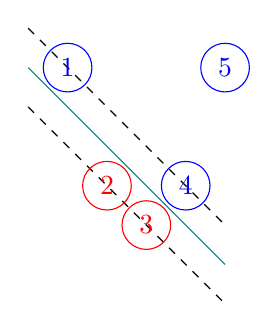
\begin{tikzpicture}
		\draw[teal] (-1.5,2) -- (1,-.5);
		
		\draw[dashed] (-1.5,1.5) -- (1,-1);
		\draw[dashed] (-1.5,2.5) -- (1,0);
		
		\node[circle,blue,draw] at (-1,2) {1};
		\node[circle,red,draw] at (-.5,0.5) {2};
		\node[circle,red,draw] at (0,0) {3};
		\node[circle,blue,draw] at (.5,0.5) {4};
		\node[circle,blue,draw] at (1,2) {5};
	\end{tikzpicture}
	\end{center}
	
	\item Si l'on retire la donnée $x_4$, qui est l'un des vecteurs de support, l'hyperplan séparateur change. Le nouvel hyperplan séparateur est parallèle à l'axe des abscisess et passe par (0,2.5), comme montré sur la figure ci-dessous. Les vecteurs $x_1$, $x_2$ et $x_3$ sont les nouveaux vecteurs de support. La nouvelle marge est $1.5$.
	
	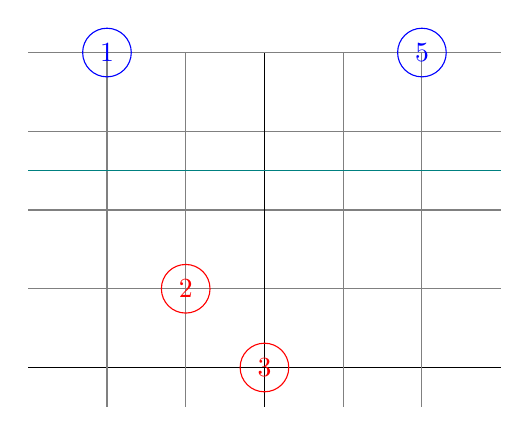
\begin{tikzpicture}
		\draw (-3,0) -- (3,0);
		
		\draw[gray] (-3,1) -- (3,1);
		\draw[gray] (-3,2) -- (3,2);
		\draw[gray] (-3,3) -- (3,3);
		\draw[gray] (-3,4) -- (3,4);
		
		\draw[gray] (-2,-0.5) -- (-2,4);
		\draw[gray] (-1,-0.5) -- (-1,4);
		\draw  (0,-0.5) -- (0,4);
		\draw[gray] (1,-0.5) -- (1,4);
		\draw[gray] (2,-0.5) -- (2,4);
		
		\draw[teal] (-3,2.5) -- (3,2.5);
		
		\node[circle,blue,draw] at (-2,4) {1};
		\node[circle,red,draw] at (-1,1) {2};
		\node[circle,red,draw] at (0,0) {3};
		\node[circle,blue,draw] at (2,4) {5};
	\end{tikzpicture}
	
	
	\end{enumerate}
	
	\end{enumerate}
	
	
	\section{Décompositions matricielles}
	
	\subsection{Valeurs propres et valeurs singulières}
	
	\begin{enumerate}
		\item On note $X = U\Sigma V^\top$ la décomposition en valeurs singulières de $X$, où $U$ et $V$ sont orthonormales et $\Sigma = \diag(\sigma_1,\ldots,\sigma_n)$ est positive. On a donc $C = XX^\top = U \Sigma^2 U^\top$ par orthonormalité de $V$.
		\begin{enumerate}
			\item  oui: la décomposition $U \Sigma^2 U^\top$ est à la fois une décomposition en valeurs propres ($U^{-1} = U^\top$) et en valeurs singulières.
			\item non: les valeurs propres de $C$ sont $\sigma_i^2$, les valeurs singulières de $X$ $\sigma_i$.
			\item oui.
		\end{enumerate}
		
		\item $C = U\Sigma^2 U^\top$ est une décomposition en valeurs propres, les vecteurs propres de $C$ sont donc les colonnes de $U$ ($CU = U\Sigma^2$). Par conséquent
		\begin{enumerate}
			\item  oui
			
			\item non: la décomposition en valeurs propres n'est pas définie pour une matrice rectangulaire
			
			\item non: : les vecteurs singuliers droits sont les colonnes de $V$. Dans le cas général, $U \neq V$.
		\end{enumerate}
	\end{enumerate}

\subsection{La SVD}

\begin{enumerate}
	\item On a
	\eq{
		C = \begin{bmatrix} 1 & 2 & 0 \\ 2 & 5 & 2 \\ 0 & 2 & 4 \end{bmatrix}.
	}
	
	\item De par la décomposition $C=XX^\top$ avec $X \in \RR^{3\times 2}$, $C$ est au plus de rang 2. Elle est en fait de rang 2 car $X$ est de rang 2.
	
	\item On vérifie pour chaque vecteur $v$ (non nul) s'il existe un réel $\la$ tel que $C v = \la v$.
	\begin{enumerate}
		\item non
		\item non
		\item oui, avec $\la=7$
		\item oui, avec $\la=3$
		\item non
		\item oui, avec $\la=0$.
	\end{enumerate}

	\item Les valeurs propres associées sont donc $7$,$3$ et $0$, et elles sont toutes positives.
	
	\item On a vu que le carré des valeurs propres de $C$ étaient les valeurs singulières de $X$ au carré. Les valeurs singulières de $X$ sont donc $+\sqrt{7}$, $+\sqrt{3}$ et $0$ (car les valeurs singulières sont toujours positives).
	
	\item On a vu que les vecteurs propres de $C$ étaient les vecteurs singuliers à gauche de $X$. On sait donc que
	\eq{
		u = \begin{bmatrix} 1\\2\\3 \end{bmatrix},
	}
	est un vecteur singulier gauche associé à la plus grande valeur singulière $\sqrt{7}$. Comme indiqué, on trouve $u_1$ en normalisant $u$:
	\eq{
		u_1 = \frac{1}{\sqrt{14}}\begin{bmatrix}1\\3\\2 \end{bmatrix}.
	}
	On détermine $v_1$ à l'aide de la deuxième indication indications:
	\eq{
		v_1 = \frac{1}{\sqrt{7}} \frac{1}{\sqrt{14}}\begin{bmatrix}0 & 1 & 2 \\1 & 2 &  0\end{bmatrix}\begin{bmatrix}1\\3\\2\end{bmatrix} = \frac{1}{7\sqrt{2}}\begin{bmatrix}7\\7\end{bmatrix} = \frac{1}{\sqrt{2}} \begin{bmatrix}1\\1\end{bmatrix} .
	}
	On en déduit finalement
	\eq{
		X_1 = \sqrt{7} \frac{1}{\sqrt{14}}\frac{1}{\sqrt{2}}\begin{bmatrix}1\\3\\2\end{bmatrix}\begin{bmatrix}1&1\end{bmatrix} = \frac{1}{2}\begin{bmatrix}1 & 1\\3 & 3\\ 2 & 2\end{bmatrix}.
	}
	
	\item On a
	\eq{
		\norm{X-X_1}_F^2 = \norm{\begin{bmatrix}-0.5 & 0.5\\-0.5 & 0.5\\1&-1\end{bmatrix}}_F^2 = 4\cdot \frac{1}{2^2} + 2 = 3.
	}
	
	NB: On retrouve $\norm{X-X_1}_F = \sqrt{3} = \sqrt{\sigma_2^2 + \sigma_3^2}$.
	
\end{enumerate}
	

\end{document}